%\usepackage[latin1]{inputenc}
\usepackage[spanish,english]{babel}
\usepackage{graphicx}
\usepackage{titling}
\usepackage[top=2.5cm, bottom=2.5cm, left=2.5cm, right=2.5cm]{geometry}
\usepackage{fix-cm}
\usepackage{xcolor}
\usepackage{titlesec}

%%%
\usepackage[final,1to1]{booklet}
\usepackage{baskervald}
\usepackage{wrapfig}
\usepackage{commath}
%%%

% TABLEOFCONTENT
\makeatletter
\def\l@subsection{\@tocline{1}{0,2pt}{2pc}{8mm}{\ \ }}
\makeatletter
\def\l@section{\@tocline{1}{0,2pt}{2pc}{8mm}{\ \ }}

% DEFINIMOS EL T�TULO
\definecolor{gray75}{gray}{0.75}
\newcommand{\hsp}{\hspace{0pt}}

\def\maketitle
{
\centering
	
\includegraphics[width=0.25\textwidth]{logo.jpg}\par\vspace{1cm}
	{\scshape\LARGE Asociaci\'on de Astronom\'ia \par}
    \vspace{0.25cm}
    {\scshape\LARGE San Fernando \par}
	\vspace{0.25cm}
	{\scshape\Large C\'adiz\par}
	\vspace{1cm}
	{\scshape\huge\thetitle \par}
	\vspace{1.5cm}
	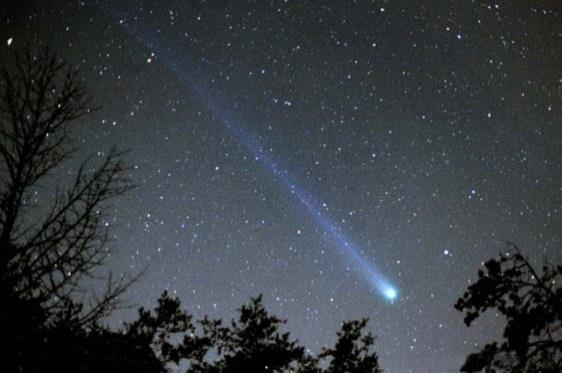
\includegraphics[width=0.75\textwidth]{portada.png}\par\vspace{1cm}
	\vfill
% Bottom of the page
	{\large \thedate\par}
    \newpage
}

\newcommand{\titulo}{\begin{titlingpage}\maketitle\end{titlingpage}}

% DEFINIMOS LOS CAP�TULOS
\titleformat{\chapter}[display]	
{\filleft}
{\color{gray75}{\filleft\small{\bfseries CAP�TULO}} {\linebreak\fontsize{90}{90}\selectfont\selectfont {\bfseries \thechapter}}}	
{2ex}
{\vspace{2ex}\bfseries \fontsize{30}{30}\selectfont}
\titlespacing{\chapter}{3mm}{*10}{15mm}[3mm]

% DEFINIMOS LAS SECCIONES
\titleformat{\section}[block]{\normalfont\Large}{\thesection}{.5em}{\bfseries}
\titlespacing*{\section}{0pt}{*4}{*1}

% DEFINIMOS LAS SUBSECCIONES
\titleformat{\subsection}[block]{\normalfont\large}{\thesubsection}{.5em}{\bfseries}
\titlespacing*{\subsection}{0pt}{*4}{*1}

% DEFINIMOS EL ABSTRACT
\newenvironment{sumario}[1][\unskip]
{
\pagestyle{empty}
\topskip0pt
\vspace*{\fill}
    \begin{center}
    \textbf{#1}
    \end{center}
}{\vspace*{\fill}\clearpage}

% DEFINIMOS LAS GEOMETR�AS DE LA P�GINA
\newcommand{\geomA}{\newgeometry{top=3.5cm, bottom=3.5cm, left=3.5cm, right=3.5cm}}
\newcommand{\geomB}{\newgeometry{top=2.5cm, bottom=2.5cm, left=2.5cm, right=2.5cm}}

% DEFINIMOS LOS AGRADECIMIENTOS
\newenvironment{agradecimientos}
{
    \newgeometry{top=3.5cm, bottom=3.5cm, left=3.5cm, right=3.5cm}
}
{
    \clearpage
    \restoregeometry
}